\section{Анализ алгоритмов и методов компьютерного зрения для извлечения признаков в антропометрии}

Использование современных методов компьютерного зрения позволяет разрабатывать новые подходы к автоматизации различных адач антропометрии. Компьютерное зрение предоставяляет большой арсенал методов для решения задач антропометрии. Условно такие задачи можно разбить на следующие этапы: калибровка, регистрация изображения (или видео), обнаружение объекта (человека), сегментация и выделение признаков (антропометрических измерений). Дополнительно может понадобиться классификация признаков и  построение 3D модели человека (это будет рассмотрено ниже) \cite{Rebak2016}.

\subsection{Антропометрические признаки}

Изображение представлено матрицей пикселей. Изображение содержит различные функции, это зависит от содержания каждого изображения. Исходя из нашей цели необходимо реализовать алгоритмы извлечения признаков, чтобы достичь наилучшей точности, устойчивости и скорости антропометрии.

Итак, первая задача состоит в использовании и преобразовании изображения в вектор признаков. По сути это представление информации в более сжатом виде в зависимости от решаемой задачи. 

Признак (feature)  $f$  объекта $a$ – отображение $f:A\rightarrow D_f$  где $D_f$ – множество допустимых значений признака \cite{Mecte2002}.  Если имеется набор признаков $f_1,…,f_n$, то вектор $x= \left(f_1\left(a\right), ..., f_n\left(a\right)\right)$ называется признаковым описанием объекта $a\in A$. Признаковые описания с определенными ограничениями допустимо отождествлять с самими объектами. При этом множество $A=\left(D_{f_1}\times ... \times D_{f_n}\right)$ называют признаковым пространством (feature space, пространство признаков). Задаче извлечения признаков объектов, как правило, предшедствуют этапы обнаружения и сегментации объектов. 
Антропометрические признаки выражены в форме и размерах частей человеческого тела (рис. \ref{img1}).
\begin{figure}[htb]
\centering
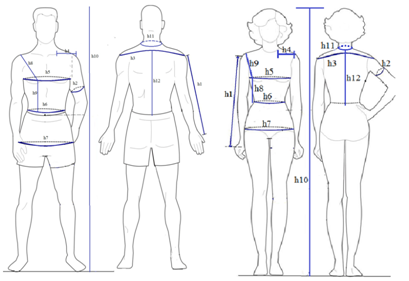
\includegraphics [scale=0.8] {images/h1.png}
\begin{center}
%\captionsetup{justification=justified, labelsep=period}
\caption{Описание антропометрических признаков.} \label{img1}
\end{center}
\end{figure}

Признаки формы. Форма объекта или области является важной характеристикой при обнаружении и классификации изображений в распознавании образов \cite{Jones2002}, \cite{Dubinskiy2003}. Основная цель анализа формы состоит в измерении геометрических свойств объекта, используемых в классификации, сравнения и распознавания объектов \cite{Kpalma2006}. Так, в области антропометрии, антрометрической характеристикой является размер частей человеческого тела. Он состоит из следующих величин \cite{urlclothes2015}: рост, длина рук, длина ног, окружность талии, окружность грудной клетки, окружность бедер и т.д. Современные антропометрические измерения могут служить основой для 3D моделей человеческого тела\cite{Toldo2009}, \cite{Ponce1989}, \cite{Zhang2001}.

Использование цвета кожи в ввиде признаков. Цвет является отличительной особенностью и используется для алгоритма обнаружения кожи \cite{Fink2006}. Каждый пиксель (информация о цвете) может быть представлен в виде трехмерной точки в определенном цветовом пространстве \cite{Albio2001}, \cite{Shin2002}. Общие цветовые пространства: RGB, Munsell, CIE, HSV \cite{Jones2002}.

\subsection{Извлечение антропометрических признаков}

Приведем краткий обзор исследований, посвященных применению методов компьютерного зрения к решению задач антропометрии, анализу положений человека и создания 3D-моделей. Для статических изображений было сделано несколько научно-исследовательских работ для того, чтобы обнаружить человеческое тело, используя описание фона и модели человеческого тела \cite{Mori2002}. В \cite{Belongie2002} представлен алгоритм сегментации частей тела на основе силуэта. Данный подход делит тело на основе использования контура каждой области на теле человека. Авторы отмечают, что их алгоритм выполняется плохо, когда части тела, особенно руки, держатся близко к телу. Авторы \cite{Mittal2003} продемонстрировали, что использование искусственно сгенерированных данных обучения помогает произвести сегментацию человеческого контура, взятого из шумных изображений реального силуэта. Авторы утверждают, что такая сегментация должна хорошо работать, несмотря на шум в исходных данных.

Извлечение антропометрических признаков выбирается на основе 2D-изображений. Оно предоставляет данные для многих приложений. Например: бесконтактное измерение размеров человеческого тела \cite{Lin2008}, построение 3D моделей \cite{Lin2010}, \cite{Lin2012}, распознавание человеческих действий \cite{Ikizler2008}. 
В работе \cite{Gopal} предложена методика сочетания наборов данных (PCD) для синтеза антропометрических баз данных на основе легкодоступной информации о значениях измерения различных областей человеческого тела. Авторы собрали такие данные для улучшения анализа перемены населения. Метод состоит из трех этапов: сбор описательной статистики о антропометрии, подгонка антропометрических моделей к этой информации, а также формирование антропометрической модели для генерации необходимых данных. Применение этой процедуры продемонстрировано на двух базах данных: военных США в конце 1980-х и японской молодежи в начале 1990-х годов. Методика является простой, легко применимой и точной. В данной статье \cite{Adams} представлен количественный анализ качества данных, собранных в ходе опроса населения волонтерами.  В результате обследования населения были получены данные артериального давления и антропометрии. На протяжении всего исследования собраны антропометрические данные и кровяное давление, которые были в пределах допуска для ошибок, установленных в начале исследования. В статье \cite{Jiang2012} предлагается подход для автоматического обнаружения ключевых точек контура человеческого тела. Этот метод применяется к изображениям, в которых имеется две раличные  позы (стоя в профиль и анфас). Реализуется он следующим образом: во-первых, используется эффективный подход к обнаружению формы тела - метод на основе обнаружения края \cite{Canny1986} и 8-связного цепного кода Фримэна \cite{Freeman1961}. Затем определяются взаимосвязанные регионы. Ряд характерных точек извлекается на основании указанных правил путем измерения разности между областями сегментов. В общей сложности 101 характерная точка с четкими геометрическими свойствами извлекаются автоматически, в том числе 27 точек, соответствующих определений ориентиров об измерениях швейной индустрии. Наконец, предлагаемый подход был протестирован на человеческих субъектах, и целых 101 характерных точек с конкретными геометрическими характеристиками были правильно извлечены, что свидетельствует об эффективной и надежной работы (рис. \ref{img2}).

\begin{figure}[ht!]
\centering
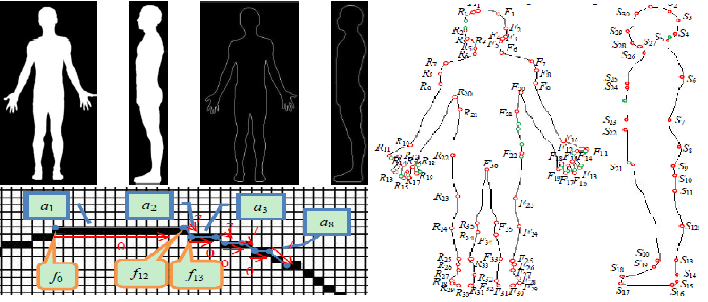
\includegraphics [scale=0.8] {images/h2.png}
\begin{center}
%\captionsetup{justification=justified, labelsep=period}
\caption{Маркировка контура в методе извлечения антропометрических признаков на основе ключевых точек \cite{Lin2008}.} \label{img2}
\end{center}
\end{figure}

В работе \cite{Nevatia2009} предложен метод обнаружения объектов в случае их частичной видимости в поле зрения. Метод апробирован на видеопотоке уличных сцен. Основной вклад этого метода включает:

\begin{itemize}
	\item Проектирование иерархии для процесса обучения путем деления признаков;
	\item Метод сегментации объектов на основе  классификатора AdaBoost.
\end{itemize}

Ioffe и Forsyth \cite{Ioffe2001} предложили методы автоматизации антропометрии, основанные на обнаружении частей тела человека. Их система подразумевает, что человек одет в специальную одежду. Определения сегментов для определения ключевых точек тела, необходимых для правильного измерения длины сегментов тела встречаются в \cite{Leva1996}. 

\begin{figure}[ht!]
\centering
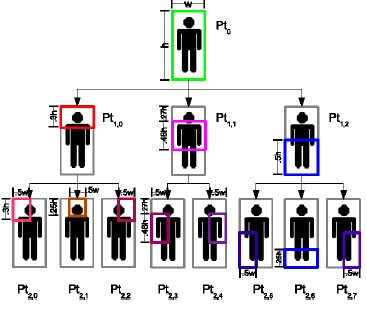
\includegraphics [scale=0.8] {images/h3.png}
\begin{center}
%\captionsetup{justification=justified, labelsep=period}
\caption{Описание системы обнаружения объекта на основе обнаружения каждой его части \cite{Nevatia2009}.} \label{img3}
\end{center}
\end{figure}

На (рис. \ref{img3}) представлена часть обнаружения тела человека на основе каскадных признаков и метода классификации на основе boosting. Программа включает в себя 3 этапа: 1) обнаружение человека, 2) обнаружение верхней части тела, средней и нижней частей тела, 3) соотнесение различных частей человеческого тела. Используется следующая классификация : верхняя часть тела (голова, правая, левая часть лица), средняя часть тела (правая рука, левая рука), нижняя часть тела (правая нога, левая нога, ноги). 

Кроме того, улучшен метод, использующий математические модели формы (3D-сканирование) для извлечения антропометрических признаков. В \cite{Baek2012} авторы предложили построение модели, которая состоит из трех основных этапов: построение базы данных, статистического анализа и генерации модели. База данных была собрана из 250 3D-сканов всего тела. Данные обрабатываются, чтобы сделать ввод данных для статистического анализа (рис. \ref{img4}). Используется соотношение частей человеческого тела для построения 3D модели. Система определяет местоположение и форму каждой части тела и вычисляет её размер. По сравнению с другими параметрическими методами моделирования человека \cite{Siebert2000}, \cite{Seo2001}, их метод вносит свой вклад путем введения нового способа соотношения формы и размеров тела путем создания усовершенствованной техники оптимизации параметров для генерации математической модели тела человека.

\begin{figure}[ht!]
\centering
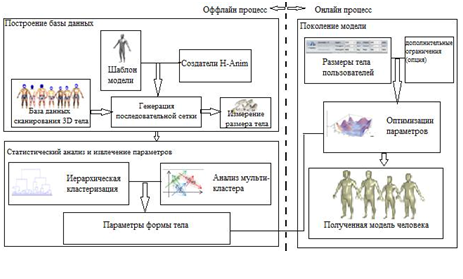
\includegraphics [scale=0.8] {images/h4.png}
\begin{center}
%\captionsetup{justification=justified, labelsep=period}
\caption{Описание метода извлечения антропометрических признаков на основе сканирования тела \cite{Baek2012}} \label{img4}
\end{center}
\end{figure}

Авторы в работе \cite{Blanz1999} также предложили метод математического моделирования формы человеческого тела. Система собирает данные путем 3D сканирования человеческого лица. Система анализирует полученные данные на основе основного метода главных компонент - PCA. Используя эту специальную базу данных, можно проанализировать и извлечь доминирующие переменные, определяющие форму лица. Используя идеи статьи \cite{Blanz1999}, Allen \cite{Allen2003} установил набор 3D данных сканирования тела. Был разработан новый способ генерации последовательной структуры сетки путем аппроксимации на основе шаблонов. В \cite{Seo2003}, \cite{Seo2004} авторы предложили использовать нейросетвой подход в этой задаче. Этот подход показал высокую эффективность для соотнесения размера фактического человеческого тела с размером тела базы данных. Критическую роль в этом подходе играет процесс обучения. Была обнаружена зависимость между формой и размерами человеческого тела. На основе этих отношений, система синтезирует новую модель с размером тела путем сопоставления формы в базе данных. Стандартные сканеры обычно используют бинарные модели, состоящие из черных и белых полос.  Этот подход подвержен ошибкам из-за зависит от разрешения и шума \cite{Rocchini2001}. Кроме того, это также зависит от расстояния между объектом и устройством. Это влияет на результаты восстановления изображения на основе данных, которые получены со сканера. Система работает эффективно даже в условиях низкой освещенности. Другой подход, основанный на компьютерном зрении изложен в работе \cite{Taeyoung2015}. Система состоит из четырех основных этапов: обработки изображений на основе вычитания фона и распознавания маркера, обработки инфракрасных изображений для надежного обнаружения маркера, для проектирования ортопедических стелек с учетом индивидуальных особенностей (рис. \ref{img5}).

\begin{figure}[ht!]
\centering
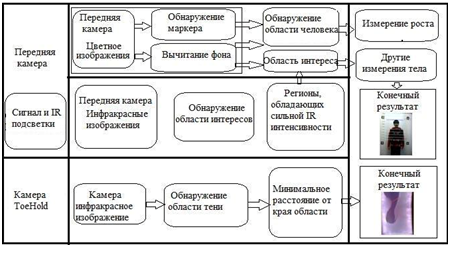
\includegraphics [scale=0.8] {images/h5.png}
\begin{center}
%\captionsetup{justification=justified, labelsep=period}
\caption{Описание системы извлечения антропометрических признаков в остеопатии\cite{Taeyoung2015}.} \label{img5}
\end{center}
\end{figure}

Эта тема получила развитие в работах \cite{McCulloch1988} и \cite{Lee2000}.
